\documentclass[12pt]{scrartcl}

% packages
\usepackage[
    a4paper, total={18cm, 26cm},
    left=0.75in,
    right=0.75in,
    top=0.75in,
    bottom=0.50in,
    footskip=15pt
]{geometry}
\usepackage{lastpage}
\usepackage{graphicx} % \includegraphics
\usepackage{amsmath} % math
\usepackage{steinmetz} % \phase
\usepackage{import} % \import
\usepackage{esdiff} % \diff
\usepackage{fancyhdr} % header and footer
\usepackage[portuguese]{babel}

% configs
\setlength{\parindent}{0pt}

% comandos
\renewcommand{\familydefault}{\sfdefault}
\newcommand{\un}[1]{\;\textrm{#1}}
\newcommand{\logo}{\quad \Rightarrow \quad}
\newcommand{\fase}[1]{\ensuremath{\phase{{#1}^{\circ}}}}

\graphicspath{ {./images/} }

\begin{document}

\numberwithin{figure}{section}
\numberwithin{equation}{section}

\pagestyle{fancy}

\fancyhead{}
\fancyhead[L]{Avaliação 2 - Algoritmo Coeficiente Convectivo}
\fancyhead[R]{EMA255 - Termodinâmica Computacional}
\fancyfoot{}
\fancyfoot[R]{Pág. \thepage \; / \pageref{LastPage}}

\begin{center}
    Aluno: Raphael Henrique Braga Leivas \\
    Matrícula: 2020028101 \\
    Professor Responsável: Márcio Ziviani \\[20pt]

    Código fonte LaTeX desse arquivo pode ser visto em meu GitHub pessoal:
\end{center}

\hrule

\section{Problema}

Precisamos criar um algoritmo para determinar a temperatura de equilíbrio da superfície
da parede esquerda $T_e$ de uma placa vertical. Temos as seguintes informações dadas:

\begin{itemize}
    \item Condutividade térmica: $k=2,5 \un{W/m$^2$K}$
    \item Comprimento: $L=5,0 \un{m}$
    \item Altura: $H=2,0 \un{m}$
    \item Espessura: $W=0,25 \un{m}$
    \item Velocidade do ar ambiente na face da parede: $u_{\infty}=3 \un{m/s}$
    \item Temperatura do ar ambiente na face da parede: $T_{\infty}=300 \un{K}$
    \item Fluxo de calor prescrito sobre a parede esquerda: $q_{p}^{''}=750 \un{W/m$^2$}$
    \item Temperatura da parede direita: $T_d=350 \un{K}$
\end{itemize}

\section{Solução}

De posse dessas informações, fazemos um desenho esquemático do problema, exibido na   
Figura \ref{fig:problemaParede}. 

\begin{figure}[h!]
    \caption{Diagrama do problema posto, com superfície de controle destacada.}
    \label{fig:problemaParede}
    \centering
    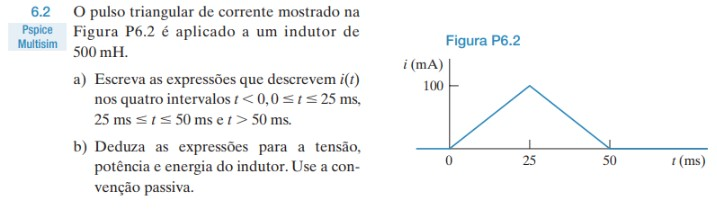
\includegraphics[scale=1.0]{problema.jpg}
    \par{Fonte: elaboração própria.}
\end{figure}

Como mostra a Figura \ref{fig:problemaParede}, temos uma superfície de controle na  
parede esquerda. Aplicando a primeira lei da termodinâmica sobre essa superfície, temos

\begin{equation}\label{eq:primeiraLei}
    \overset{\cdot}{E}_{in} + \overset{\cdot}{E}_{g} - \overset{\cdot}{E}_{out} = \overset{\cdot}{E}_{st}
\end{equation}

Como temos uma superfície de controle, não há energia armazenada e energia gerada. Além disso, no modelo
da Figura \ref*{fig:problemaParede}, repare que todos os fluxos de calor estão entrando na superfície, de tal  
maneira que $\overset{\cdot}{E}_{out} = 0$. Assim, \eqref{eq:primeiraLei} se reduz a 

\begin{equation}\label{eq:primeiraLeiReduzida}
    \overset{\cdot}{E}_{in} = 0
\end{equation}

Expandindo o termo $\overset{\cdot}{E}_{in}$, 

\[ q_{p}^{''} + q_{c}^{''} + q_{k}^{''} = 0 \]

\[ q_{p}^{''} + h_c\left(T_{\infty}-T_e\right) + \frac{k}{L}\left(T_d-T_e\right) = 0 \]

Isolando o coeficiente convectivo $h_c$, temos

\[ h_c\left(T_{\infty}-T_e\right) = - q_{p}^{''} - \frac{k}{L}\left(T_d-T_e\right)\]

\begin{equation}\label{eq:hc}
    h_c = - \frac{q_{p}^{''} + \frac{k}{L}\left(T_d-T_e\right)}{T_{\infty}-T_e}
\end{equation}

Como a velocidade do ar ambiente na face da parede é $u_{\infty}=3 \un{m/s}$, temos que isso equivale a 
$10,8 \un{km/h}$ e não pode ser desprezado, de tal maneira que a convecção na face esquerda da parede é forçada.


\end{document}